\chapter{Thảo luận}

Chương này tiến hành thảo luận và phân tích chuyên sâu về các giới hạn mô hình thông qua phân bố sai số dự đoán. Nội dung chương tập trung bóc tách lỗi của hai cấu hình đạt hiệu năng cao nhất: mô hình học máy kết hợp đặc trưng thủ công (\texttt{MLP + HOG | Ảnh gốc}) và mô hình học sâu (\texttt{CNN | Ảnh gốc — Xám}). Quá trình phân tích được thực hiện trên các chiều nhân khẩu học (độ tuổi, giới tính, chủng tộc) kết hợp với việc đối chiếu chiến lược huấn luyện, từ đó cung cấp căn cứ định lượng về đặc tính học biểu diễn của từng kiến trúc. Phần cuối của chương sẽ đánh giá ảnh hưởng của phương pháp giảm chiều dữ liệu PCA đến hiệu năng và chi phí tính toán.

\section{Phân tích phân bố sai số tổng quan}
Đánh giá mức độ phân tán của sai số dự đoán so với nhãn thực tế giúp xác định các xu hướng chệch mang tính hệ thống của mô hình.

\begin{figure}[H]
    \centering
    \begin{minipage}{0.48\textwidth}
        \centering
        % [NOTE]: Chèn file ảnh Scatter của MLP+HOG Original (image_5841fb.png)
        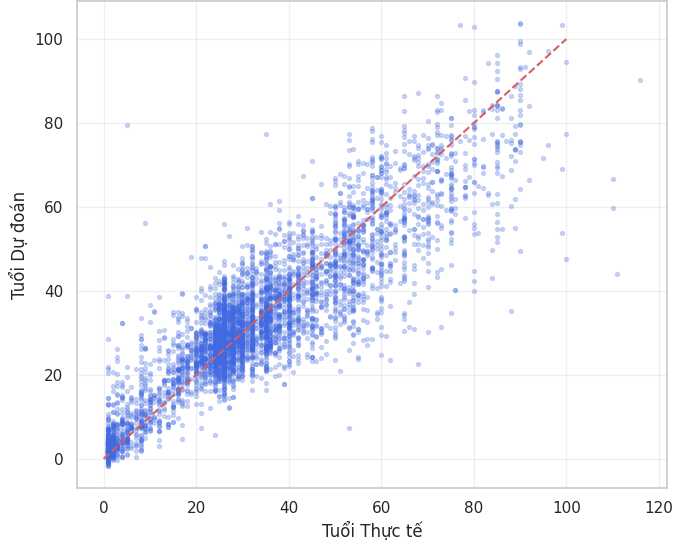
\includegraphics[width=\linewidth]{images/scatter_mlp_hog_orig.png} 
        \caption*{a) MLP + HOG | Ảnh gốc}
    \end{minipage}\hfill
    \begin{minipage}{0.48\textwidth}
        \centering
        % [NOTE]: Chèn file ảnh Scatter của CNN Original Xám (image_585f65.png)
        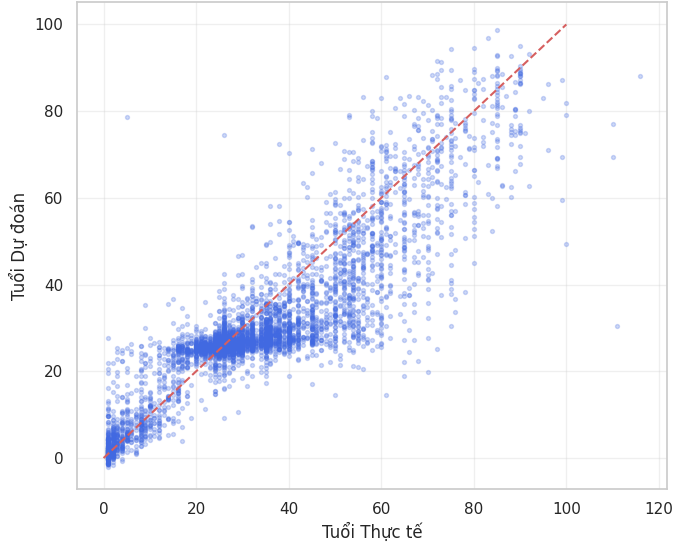
\includegraphics[width=\linewidth]{images/scatter_cnn_gray_orig.png}
        \caption*{b) CNN | Ảnh gốc — Xám}
    \end{minipage}
    \caption{Biểu đồ phân tán giữa tuổi dự đoán và tuổi thực tế của hai cấu hình tối ưu.}
    \label{fig:scatter-comparison}
\end{figure}

Hình~\ref{fig:scatter-comparison} thể hiện rõ hiện tượng phương sai thay đổi ở cả hai mô hình, trong đó biên độ sai số mở rộng dạng phễu khi độ tuổi tăng lên. Tại nhóm tuổi từ 20 đến 40, mạng CNN ép các điểm dự đoán bám sát đường chéo tham chiếu với mật độ đặc hơn đáng kể so với MLP, thể hiện năng lực tối ưu hóa cục bộ vượt trội trên vùng dữ liệu đa số. Ở dải độ tuổi cao (trên 60 tuổi), cả hai kiến trúc đều mắc phải xu hướng dự đoán thấp hơn tuổi thật. Tuy nhiên, các điểm dự đoán của CNN ít bị phân kỳ sâu xuống dưới biên độ so với tổ hợp MLP + HOG.

\section{Phân tích sai số theo đặc trưng nhân khẩu học}
\subsection{Phân tích theo nhóm tuổi}
Việc lượng hóa sai số tuyệt đối trung bình ($MAE$) theo từng phân khúc tuổi rời rạc làm bộc lộ khả năng xấp xỉ đặc trưng lão hóa của từng phương pháp. Số liệu đối chiếu được trình bày tại Bảng~\ref{tab:error-by-age}.

\begin{table}[H]
    \centering
    \footnotesize
    \renewcommand{\arraystretch}{1.5}
    \caption{So sánh sai số dự đoán (MAE) theo từng nhóm tuổi giữa MLP và CNN.}
    \label{tab:error-by-age}
    \begin{tabular}{c|ccccccccc}
        \toprule
        \textbf{Mô hình} & \textbf{0-5} & \textbf{6-12} & \textbf{13-20} & \textbf{21-30} & \textbf{31-40} & \textbf{41-50} & \textbf{51-60} & \textbf{61-80} & \textbf{80+} \\
        \midrule
        \textbf{MLP + HOG} & 3.62 & 5.90 & \textbf{5.77} & 4.98 & \textbf{6.02} & \textbf{7.65} & \textbf{9.58} & \textbf{11.03} & 15.48 \\
        \textbf{CNN (Xám)} & \textbf{3.02} & \textbf{4.94} & 6.21 & \textbf{2.40} & 7.07 & 11.91 & 13.69 & 13.09 & \textbf{12.12} \\
        \bottomrule
    \end{tabular}
\end{table}

Bảng thống kê xác nhận hai thái cực hiệu năng khác biệt giữa học máy truyền thống và học sâu:
\begin{itemize}
    \item \textbf{Khả năng tối ưu hóa vùng đa số:} Tại nhóm thanh niên (21-30 tuổi), CNN giảm sai số xuống mức cực tiểu là 2.40 tuổi (chỉ bằng một nửa so với mức 4.98 của MLP). Các bộ lọc tích chập học được biểu diễn đặc trưng xấp xỉ hoàn hảo cho phân khúc có tần suất xuất hiện dày đặc nhất trong tập dữ liệu.
    \item \textbf{Khả năng tổng quát hóa ở giới hạn độ tuổi:} Đối với cấu hình MLP, sai số tăng tuyến tính và chạm đỉnh tại nhóm người rất già (80+) với $MAE = 15.48$. Ngược lại, mạng CNN đạt đỉnh sai số ở dải 51-60 tuổi (13.69) nhưng lại giảm xuống còn 12.12 ở nhóm 80+. Về mặt lý thuyết xấp xỉ, các lớp tích chập sâu tự động trích xuất được các đặc trưng phân cấp liên quan đến thoái hóa cấu trúc xương và nếp nhăn sâu, duy trì tính bền vững cao hơn bộ mô tả định hướng gradient (HOG) khi đối mặt với sự biến thiên phức tạp của tuổi già.
\end{itemize}

\subsection{Phân tích mức độ thiên lệch theo giới tính}
Mức độ công bằng của mô hình được đánh giá qua độ chênh lệch sai số giữa các giới tính sinh học (Bảng~\ref{tab:error-by-gender}).

\begin{table}[H]
    \centering
    \footnotesize
    \renewcommand{\arraystretch}{1.2}
    \caption{So sánh sai số dự đoán (MAE) theo giới tính.}
    \label{tab:error-by-gender}
    \begin{tabular}{l|cc|c}
        \toprule
        \textbf{Mô hình} & \textbf{Nữ (Female)} & \textbf{Nam (Male)} & \textbf{Độ chênh lệch ($\Delta$)} \\
        \midrule
        \textbf{MLP + HOG} & 6.35 & 6.63 & \textbf{0.28} \\
        \textbf{CNN (Xám)} & 6.16 & 7.01 & 0.85 \\
        \bottomrule
    \end{tabular}
\end{table}

Tổ hợp \texttt{MLP + HOG} thể hiện tính ổn định cao với độ chênh lệch chỉ 0.28 tuổi. Đặc trưng HOG khai thác thông tin từ hướng của các dải biên gradient, từ đó triệt tiêu được các yếu tố nhiễu về cường độ sáng bề mặt. Ngược lại, mạng CNN hoạt động trên ảnh xám bộc lộ thiên lệch giới tính rõ rệt hơn ($\Delta = 0.85$). Khi loại bỏ thông tin đa kênh (RGB sang Grayscale), mô hình mạng nơ-ron gặp khó khăn trong việc phân tách các vùng kết cấu có độ tương phản thấp (điển hình như bóng đổ của râu quai nón ở nam giới so với nếp nhăn viền cằm), dẫn đến sự suy giảm độ chính xác cục bộ đối với ảnh nam giới.

\subsection{Phân tích phân tán theo chủng tộc}
\begin{figure}[H]
    \centering
    \begin{minipage}{0.95\textwidth}
        \centering
        % [NOTE]: Chèn file Violin của MLP+HOG Original (image_58421b.png)
        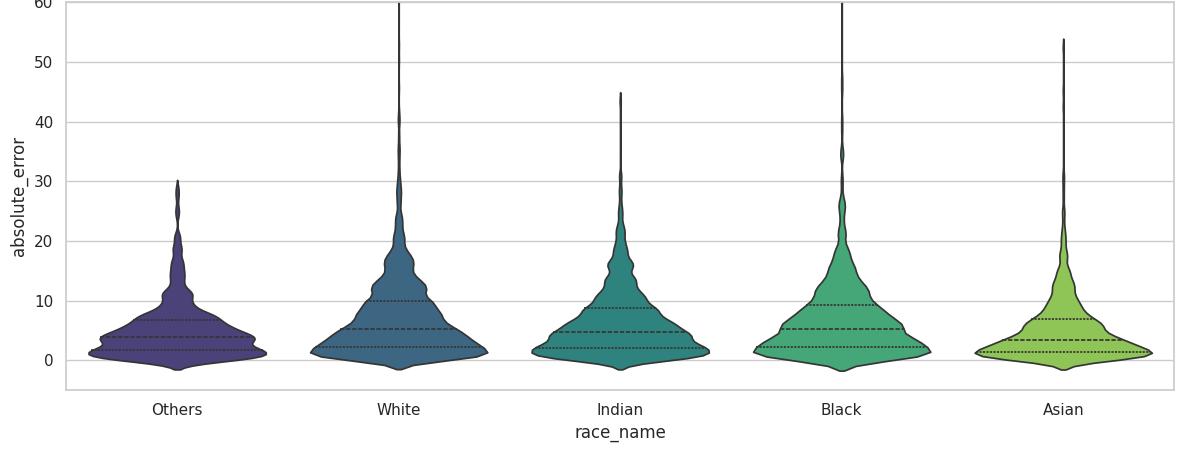
\includegraphics[width=\linewidth]{images/violin_mlp_hog_orig.png} 
        \caption*{a) MLP + HOG | Ảnh gốc}
    \end{minipage}
    
    \vspace{0.6cm} % Khoảng cách dọc giữa hai biểu đồ
    
    \begin{minipage}{0.95\textwidth}
        \centering
        % [NOTE]: Chèn file Violin của CNN Original Xám (image_585f88.png)
        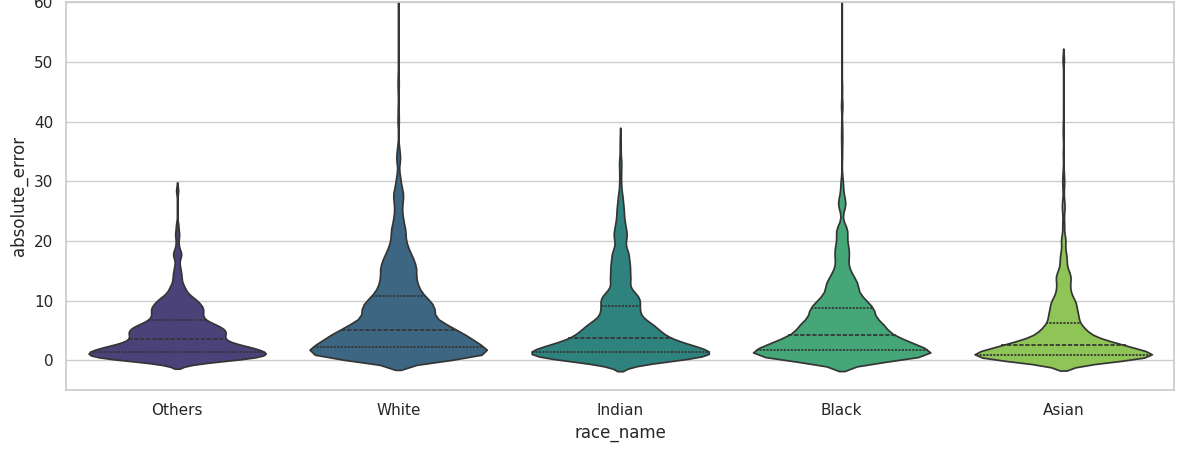
\includegraphics[width=\linewidth]{images/violin_cnn_gray_orig.png}
        \caption*{b) CNN | Ảnh gốc — Xám}
    \end{minipage}
    
    \caption{Mật độ phân tán sai số (MAE) trên từng nhóm chủng tộc.}
    \label{fig:violin-race}
\end{figure}

Biểu đồ mật độ phân bố (Hình~\ref{fig:violin-race}) xác nhận sự tồn tại của lỗi đuôi dài tại hai chủng tộc White và Black ở cả hai kiến trúc, nơi xuất hiện các điểm ngoại lai có sai số tuyệt đối xấp xỉ 50-60 tuổi. Đây là giới hạn mang tính hệ thống bắt nguồn từ ranh giới biểu diễn của tập dữ liệu. Tuy nhiên, đối với các nhóm Asian, Indian và Others, mạng CNN ép thành công mật độ phân bố đáy tiến sát về ngưỡng 0, tạo ra cấu trúc phân bố hẹp hơn đáng kể so với MLP. Mặc dù vậy, hệ quả của quá trình tối ưu hóa này là sự xuất hiện rải rác của các điểm dị biệt đột biến ở mạng học sâu.

\section{Đánh giá chiến lược huấn luyện Chung và Riêng rẽ}
Nhằm kiểm chứng giả thuyết về tính phổ quát của đặc điểm lão hóa, một thực nghiệm đối chiếu được thiết lập để so sánh Hệ số xác định ($R^2$) giữa mô hình huấn luyện trên toàn bộ dữ liệu (\textit{Chung}) và các mô hình huấn luyện độc lập trên từng phân mảnh dữ liệu chủng tộc (\textit{Riêng rẽ}). Thực nghiệm này được tiến hành trên cấu hình \texttt{MLP + HOG}.

\begin{figure}[H]
    \centering
    % [NOTE]: Chèn file Bar chart R2 của MLP+HOG Original (image_584235.png)
    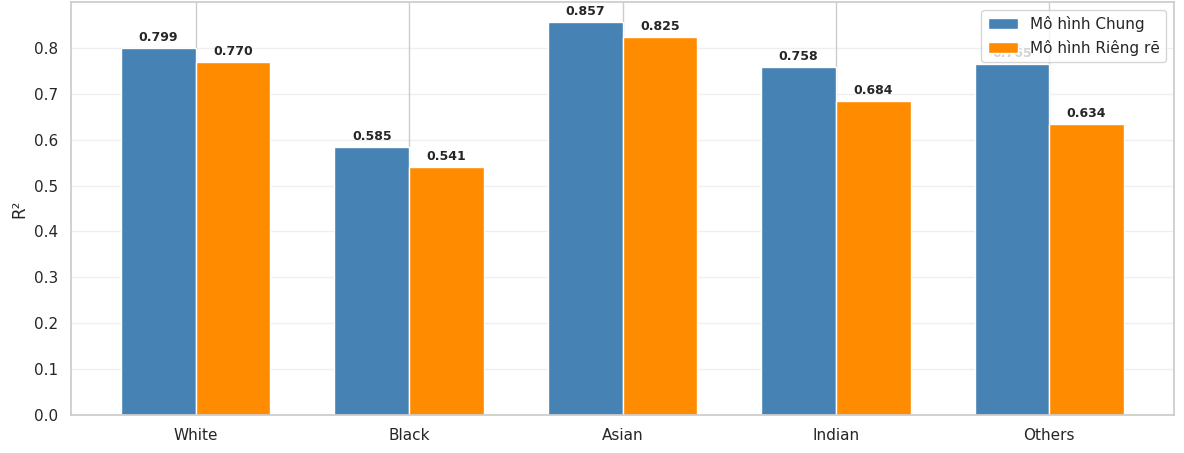
\includegraphics[width=1\linewidth]{images/r2_training_strategy.png}
    \caption{So sánh khả năng giải thích dữ liệu ($R^2$) giữa chiến lược huấn luyện Chung và Riêng rẽ.}
    \label{fig:error-training-strategy}
\end{figure}

Phân tích Hình~\ref{fig:error-training-strategy} khẳng định mô hình được huấn luyện toàn cục áp đảo hoàn toàn các mô hình phân mảnh ở mọi tập thử nghiệm. Mức sụt giảm cực đại xảy ra ở nhóm Others ($R^2$ giảm từ 0.755 xuống 0.634) và nhóm Indian ($R^2$ giảm từ 0.758 xuống 0.684). Về mặt học máy, quá trình biến đổi cấu trúc khuôn mặt theo thời gian mang tính phổ quát sinh học. Việc phân tách tập dữ liệu để huấn luyện riêng lẻ không cung cấp thêm các đặc trưng chuyên biệt cho từng chủng tộc, mà ngược lại, làm suy giảm nghiêm trọng không gian mẫu, dẫn đến hiện tượng quá khớp và làm giảm độ vững chãi của mặt phẳng hồi quy.

% \section{Phân tích khả năng giảm chiều dữ liệu}
% \label{sec:pca_analysis}
% Đặc trưng HOG có số chiều lớn, làm tăng thời gian tính toán của các mô hình như SVR và Random Forest. Phương pháp Phân tích Thành phần Chính (PCA) được sử dụng để giảm số chiều vector xuống các mức từ 10 đến 400 chiều.

% \begin{sidewaysfigure}
% 	\centering
% 	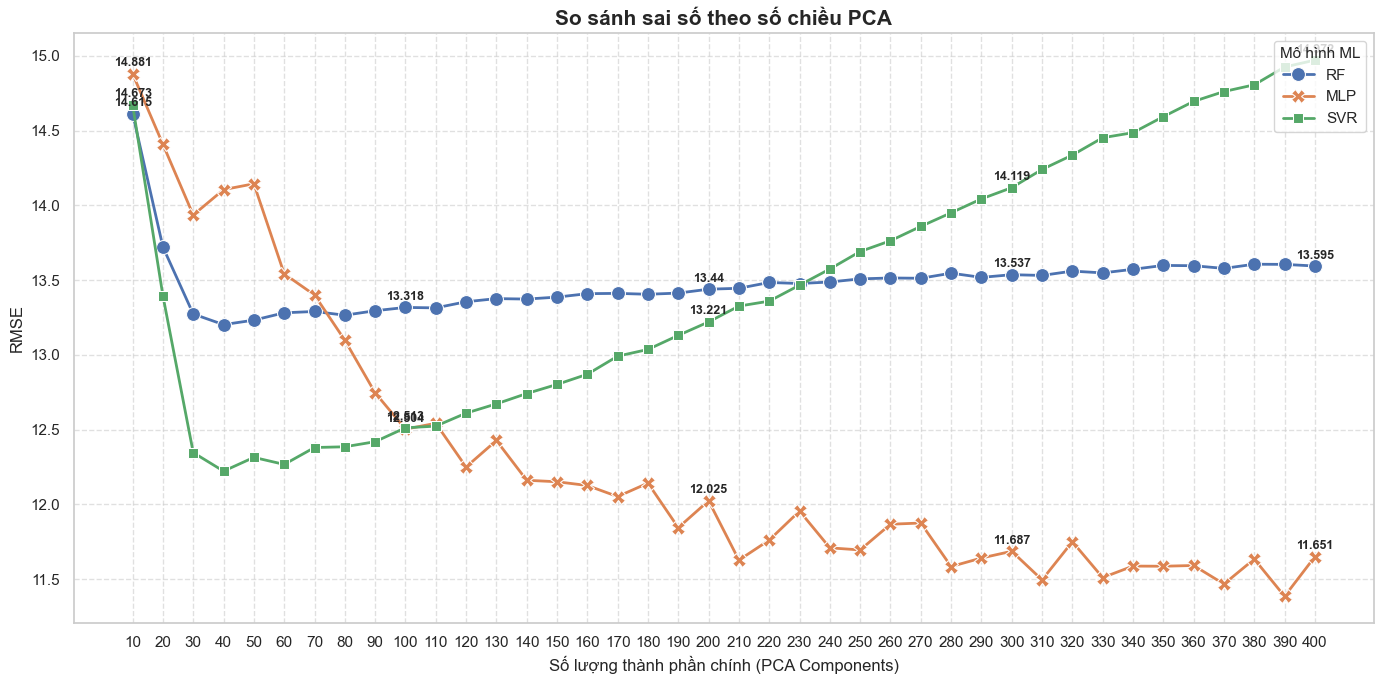
\includegraphics[width=1\linewidth]{images/error_PCA.png}
% 	\caption{So sánh sai số RMSE theo số lượng thành phần chính (PCA) trên 3 mô hình.}
% 	\label{fig:error-pca}
% \end{sidewaysfigure}

% \begin{table}[H]
% 	\centering
% 	\caption{Đánh giá RMSE của các mô hình theo mức độ giảm chiều PCA.}
% 	\label{tab:pca-results}
% 	\resizebox{\linewidth}{!}{
% 		\begin{tabular}{rccc | rccc}
% 			\toprule
% 			\textbf{Số chiều} & \textbf{MLP} & \textbf{RF} & \textbf{SVR} & \textbf{Số chiều} & \textbf{MLP} & \textbf{RF} & \textbf{SVR} \\
% 			\midrule
% 			10 & 14.881 & 14.615 & 14.673 & 210 & 11.628 & 13.446 & 13.327 \\
% 			20 & 14.409 & 13.722 & 13.395 & 220 & 11.762 & 13.485 & 13.360 \\
% 			30 & 13.936 & 13.274 & 12.347 & 230 & 11.956 & 13.478 & 13.467 \\
% 			40 & 14.106 & 13.203 & \textbf{12.223} & 240 & 11.710 & 13.488 & 13.575 \\
% 			50 & 14.145 & 13.233 & 12.315 & 250 & 11.696 & 13.509 & 13.692 \\
% 			60 & 13.543 & 13.282 & 12.268 & 260 & 11.868 & 13.515 & 13.764 \\
% 			70 & 13.401 & 13.291 & 12.381 & 270 & 11.876 & 13.513 & 13.860 \\
% 			80 & 13.099 & 13.266 & 12.386 & 280 & 11.585 & 13.547 & 13.951 \\
% 			90 & 12.747 & 13.296 & 12.420 & 290 & 11.642 & 13.519 & 14.044 \\
% 			100 & 12.504 & 13.318 & 12.513 & 300 & 11.687 & 13.537 & 14.119 \\
% 			110 & 12.543 & 13.315 & 12.524 & 310 & 11.496 & 13.532 & 14.241 \\
% 			120 & 12.251 & 13.356 & 12.611 & 320 & 11.751 & 13.561 & 14.337 \\
% 			130 & 12.428 & 13.377 & 12.673 & 330 & 11.511 & 13.549 & 14.453 \\
% 			140 & 12.162 & 13.374 & 12.742 & 340 & 11.588 & 13.573 & 14.487 \\
% 			150 & 12.152 & 13.387 & 12.803 & 350 & 11.587 & 13.599 & 14.594 \\
% 			160 & 12.127 & 13.410 & 12.871 & 360 & 11.592 & 13.597 & 14.696 \\
% 			170 & 12.053 & 13.412 & 12.992 & 370 & 11.468 & 13.579 & 14.762 \\
% 			180 & 12.143 & 13.406 & 13.037 & 380 & 11.635 & 13.607 & 14.807 \\
% 			190 & 11.845 & 13.414 & 13.131 & 390 & \textbf{11.386} & 13.606 & 14.926 \\
% 			200 & 12.025 & 13.440 & 13.221 & 400 & 11.651 & 13.595 & 14.972 \\
% 			\midrule
% 			\multicolumn{4}{c|}{} & \textbf{Gốc (8100D)} & \textbf{9.570} & 13.250 & 12.650 \\
% 			\bottomrule
% 		\end{tabular}
% 	}
% \end{table}

% Dựa trên dữ liệu từ Hình~\ref{fig:error-pca} và Bảng~\ref{tab:pca-results}:
% \begin{itemize}
% 	\item \textbf{Mô hình SVR:} SVR không dùng PCA đạt RMSE 12.65. Khi nén PCA xuống 40 chiều, RMSE của SVR giảm xuống mức tối ưu là 12.223. Đồ thị Hình~\ref{fig:error-pca} cho thấy đường biểu diễn của SVR đạt đáy tại 40 chiều và tăng dần khi số chiều cao hơn. PCA loại bỏ nhiễu và thông tin thừa, giúp SVR hoạt động chính xác và nhanh hơn đáng kể.
% 	\item \textbf{Mô hình Random Forest:} Đường biểu diễn của RF đi ngang ở mức 13.2 đến 13.6 từ mốc 40 chiều trở đi, tương tự như khi dùng dữ liệu gốc. PCA không làm thay đổi lớn hiệu năng của mô hình này do bản chất cấu trúc cây quyết định (decision tree) đã bao gồm khả năng chọn lọc đặc trưng.
% 	\item \textbf{Mô hình MLP:} MLP có xu hướng giảm dần sai số khi số lượng thành phần chính tăng lên và đạt mức tốt nhất là 11.386 tại 390 chiều. Tuy nhiên, kết quả này vẫn kém xa so với RMSE 9.570 khi sử dụng dữ liệu nguyên bản chưa nén. Khác với SVR, kiến trúc mạng nơ-ron đa tầng có khả năng tự động trích xuất các đặc trưng phi tuyến ẩn sâu từ dữ liệu thô cực kỳ tốt. Việc nén dữ liệu bằng phép chiếu tuyến tính như PCA trước khi đưa vào MLP đã vô tình loại bỏ nhiều thông tin quan trọng.
% \end{itemize}

% \section{Tổng kết chương}
% Chương này đã đi sâu vào thảo luận và phân tích các nguyên nhân gây ra sai lệch của mô hình dự đoán. Kết quả chỉ ra rằng sự thiếu hụt dữ liệu và độ phân tán lớn về đặc điểm lão hóa là nguyên nhân chính khiến mô hình gặp khó khăn với người cao tuổi và các chủng tộc thiểu số. Đồng thời, qua thực nghiệm giảm chiều dữ liệu, PCA được chứng minh là hữu ích để tối ưu thời gian tính toán cho mô hình học máy truyền thống như SVR, trong khi lại làm suy giảm đáng kể hiệu năng của mạng nơ-ron (MLP) do làm mất đi các thông tin phi tuyến quan trọng.


\section{Phân tích khả năng giảm chiều dữ liệu}
\label{sec:pca_analysis}
Đặc trưng HOG nguyên bản sở hữu số chiều rất lớn (8100 chiều), gây ra hiện tượng thắt cổ chai tính toán đối với các thuật toán học máy truyền thống như SVR và Random Forest. Phương pháp Phân tích thành phần chính (PCA) được áp dụng để nén không gian đặc trưng xuống các mức từ 10 đến 400 chiều, nhằm đánh giá sự đánh đổi giữa hiệu năng (thông qua hệ số $R^2$) và chi phí tính toán.

\begin{sidewaysfigure}
	\centering
	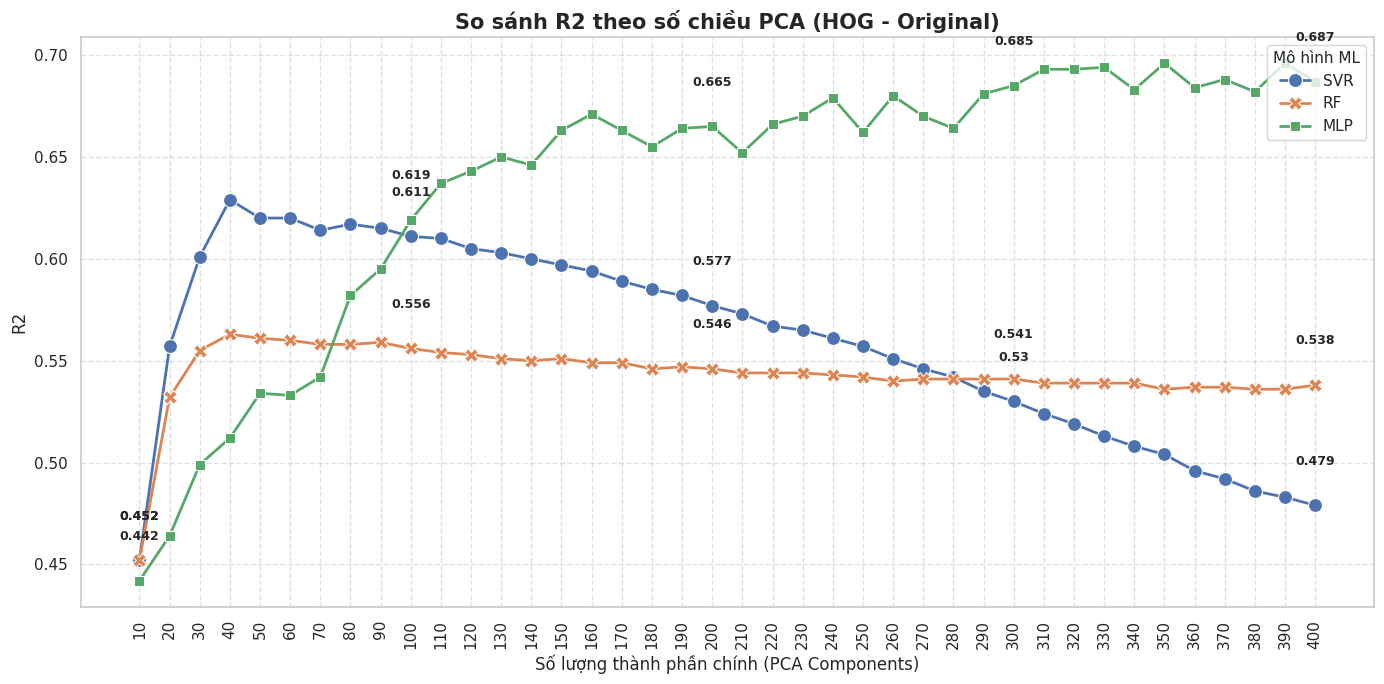
\includegraphics[width=1\linewidth]{images/pca_r2_comparison.png}
    \caption{So sánh hệ số xác định ($R^2$) của các mô hình theo số lượng thành phần chính (PCA).}
	\label{fig:r2-pca}
\end{sidewaysfigure}

\begin{table}[H]
    \centering
    \footnotesize
    \renewcommand{\arraystretch}{1.1}
    \caption{Đánh giá hệ số xác định ($R^2$) của các mô hình theo mức độ giảm chiều PCA.}
    \label{tab:pca-results}
    \resizebox{\linewidth}{!}{
        \begin{tabular}{rccc | rccc}
            \toprule
            \textbf{Số chiều} & \textbf{MLP} & \textbf{RF} & \textbf{SVR} & \textbf{Số chiều} & \textbf{MLP} & \textbf{RF} & \textbf{SVR} \\
            \midrule
            10 & 0.442 & 0.452 & 0.452 & 210 & 0.652 & 0.544 & 0.573 \\
            20 & 0.464 & 0.532 & 0.557 & 220 & 0.666 & 0.544 & 0.567 \\
            30 & 0.499 & 0.555 & 0.601 & 230 & 0.670 & 0.544 & 0.565 \\
            40 & 0.512 & \textbf{0.563} & \textbf{0.629} & 240 & 0.679 & 0.543 & 0.561 \\
            50 & 0.534 & 0.561 & 0.620 & 250 & 0.662 & 0.542 & 0.557 \\
            60 & 0.533 & 0.560 & 0.620 & 260 & 0.680 & 0.540 & 0.551 \\
            70 & 0.542 & 0.558 & 0.614 & 270 & 0.670 & 0.541 & 0.546 \\
            80 & 0.582 & 0.558 & 0.617 & 280 & 0.664 & 0.541 & 0.542 \\
            90 & 0.595 & 0.559 & 0.615 & 290 & 0.681 & 0.541 & 0.535 \\
            100 & 0.619 & 0.556 & 0.611 & 300 & 0.685 & 0.541 & 0.530 \\
            110 & 0.637 & 0.554 & 0.610 & 310 & 0.693 & 0.539 & 0.524 \\
            120 & 0.643 & 0.553 & 0.605 & 320 & 0.693 & 0.539 & 0.519 \\
            130 & 0.650 & 0.551 & 0.603 & 330 & 0.694 & 0.539 & 0.513 \\
            140 & 0.646 & 0.550 & 0.600 & 340 & 0.683 & 0.539 & 0.508 \\
            150 & 0.663 & 0.551 & 0.597 & 350 & 0.696 & 0.536 & 0.504 \\
            160 & 0.671 & 0.549 & 0.594 & 360 & 0.684 & 0.537 & 0.496 \\
            170 & 0.663 & 0.549 & 0.589 & 370 & 0.688 & 0.537 & 0.492 \\
            180 & 0.655 & 0.546 & 0.585 & 380 & 0.682 & 0.536 & 0.486 \\
            190 & 0.664 & 0.547 & 0.582 & 390 & \textbf{0.696} & 0.536 & 0.483 \\
            200 & 0.665 & 0.546 & 0.577 & 400 & 0.687 & 0.538 & 0.479 \\
            \midrule
            \multicolumn{4}{c|}{\textbf{Dữ liệu gốc (8100 chiều)}} & \textbf{0.792} & 0.591 & 0.626 \\
            \bottomrule
        \end{tabular}
    }
\end{table}

Dữ liệu từ Hình~\ref{fig:r2-pca} và Bảng~\ref{tab:pca-results} cho thấy sự khác biệt về đặc tính học biểu diễn của ba thuật toán khi áp dụng phương pháp giảm chiều dữ liệu:
\begin{itemize}
    \item \textbf{Hồi quy Vector hỗ trợ (SVR):} Mô hình đạt giá trị $R^2 = 0.629$ tại mốc 40 thành phần chính. Kết quả này cao hơn hiệu năng khi huấn luyện trên toàn bộ 8100 chiều gốc ($R^2 = 0.626$). Khi tiếp tục tăng số chiều, $R^2$ của SVR có xu hướng giảm. Điều này cho thấy PCA có tác dụng lọc nhiễu, loại bỏ các đặc trưng gradient không mang nhiều thông tin, từ đó hỗ trợ hàm nhân RBF của SVR xác định mặt phẳng phân cách tối ưu hơn.
    \item \textbf{Rừng ngẫu nhiên (Random Forest):} Hiệu năng của RF tăng ở các mốc đầu và đạt đỉnh cục bộ $R^2 = 0.563$ tại 40 chiều, sau đó duy trì ổn định. Tuy nhiên, mức hiệu năng này vẫn thấp hơn so với khi sử dụng dữ liệu gốc ($R^2 = 0.591$). Do cấu trúc cây quyết định phân nhánh dựa trên các ngưỡng của từng đặc trưng độc lập, phép biến đổi tổ hợp tuyến tính của PCA làm thay đổi không gian đặc trưng ban đầu, dẫn đến việc mô hình RF suy giảm hiệu năng khi áp dụng giảm chiều.
    \item \textbf{Mạng nơ-ron đa tầng (MLP):} Ngược lại với SVR, hiệu năng của MLP có xu hướng tăng theo số lượng thành phần chính, đạt $R^2 = 0.696$ tại các mốc 350 và 390 chiều. Dù vậy, kết quả này vẫn thấp hơn khoảng 0.1 so với mô hình gốc 8100 chiều ($R^2 = 0.792$). Mạng nơ-ron vốn có khả năng tự động trích xuất các đặc trưng phi tuyến từ dữ liệu thô. Việc áp dụng phép chiếu tuyến tính như PCA làm mất đi một phần thông tin vi mô của ảnh, từ đó làm giảm khả năng xấp xỉ hàm mục tiêu của kiến trúc MLP.
\end{itemize}

\section{Tổng kết chương}
Chương 4 đã phân tích định lượng các giới hạn của hệ thống dự đoán tuổi. Đánh giá phân bố sai số cho thấy các mô hình đạt độ chính xác cao nhất ở nhóm tuổi thanh niên, nhưng độ lỗi tăng ở nhóm người cao tuổi do phương sai của đặc điểm lão hóa lớn. Phân tích cũng chỉ ra kiến trúc CNN có khả năng xấp xỉ tốt hơn đối với các đặc trưng lão hóa phức tạp, trong khi cấu hình \texttt{MLP + HOG} cho kết quả đồng đều hơn giữa hai nhóm giới tính. Bên cạnh đó, thực nghiệm PCA chứng minh rằng việc giảm chiều dữ liệu là phương pháp hiệu quả để khử nhiễu và tăng hiệu năng cho mô hình SVR, nhưng lại gây mất mát thông tin và làm giảm độ chính xác đối với mô hình phi tuyến như mạng MLP.